\section{Retrieving Images in Clusters}
\label{sec_introduction}

\todo{introduce the introduction?}

\subsection{Problem Statement \& Motivation}
Many semantic image analysis algorithms, e.g. for image categorization or content detection, require training data on which the relevant features can be learned. Obtaining such training data can be a troublesome task, especially when the training set is created manually from scratch. If, for example, an algorithm shall be trained to identify and categorize kinds of food, one would have to think of all possible kinds of food, search for corresponding images and divide them into homogeneous groups. \\
A good place to search for images are online photo communities like Flickr\footnote{https://www.flickr.com/}, which provide vast amounts of collaboratively tagged images. These communities are also called folksonomies\index{Folksonomy}, i.e. socially indexed collections.
Although folksonomies can be good sources for training data due to the semantic metadata that tags provide, several problems exist: First of all, annotations are often of poor quality, since anyone can tag anything without any control mechanisms. Secondly, one can only search for a specific term, and will obtain images for all of the term's meanings, while on the other hand the retrieval is limited to those images which are annotated with the exact same tag. This results to the fact, that usually no semantically relations to other terms are provided. Furthermore, the images will be of a very large visual diversity, which is often not desired. \\

This work presents a tool whose main aim is to create homogeneous groups of semantically and visually similar pictures for a given topic in order to aid with the laborious assembly of training and test data sets. It is based on the 1 million images of the MIRFLICKR-1M\footnote{http://press.liacs.nl/mirflickr/} file set, and addresses the above mentioned difficulties. The main challenges encountered were homonymy\index{Homonymy} of keywords (the fact that one word can have multiple meanings), low quality of tags and other annotations, and the consideration of both semantic and visual information about a picture.

\subsection{Clustered Tree Nodes Approach}
The tool has been implemented as a Python web application, using WordNet\footnote{http://wordnet.princeton.edu/} for semantic image analysis, SimpleCV\footnote{http://www.simplecv.org/} for visual image analysis and Flask\footnote{http://flask.pocoo.org/} for the frontend presentation.\\
It provides ready-to-use semantically and visually homogeneous image clusters for a given topic, or search term. This is achieved by 2 major phases: First, spanning a tree of subordinate terms of the topic and retrieving related images by their keywords for each node of the tree. Second, clustering the images by their predominant keywords as well as by colors and edge structure. The following figure \ref{fig_overallprocess} illustrates these two main phases of the tool.

\begin{figure}[h]
\centering
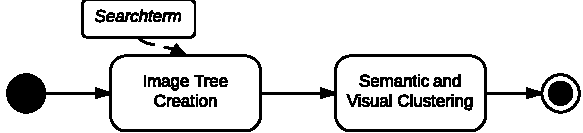
\includegraphics[]{images/search_process_highlevel.pdf}
\caption{The two main phases of the clustered image search}
\label{fig_overallprocess}
\end{figure}

\bigskip

After giving an overview of Related Work in chapter 2, we present how we analyze the image annotations and the user's search term to retrieve relevant images in chapter 3. The methods applied to cluster the images semantically and visually are described in chapter 4. Chapter 5 explains how we evaluate our approach, while the evaluation results are discussed in chapter 6. At last, chapter 7 gives ideas for improvement and possible future work.
